\section{Fundamentação teórica}

\begin{frame}{Sistema de arquivos distribuído}
	%\textbf{Sistema de arquivos distribuído}
	\begin{itemize}
		\item Conjunto de vários servidores distribuídos fisicamente, conectados através de redes locais ou internet.
		\item Voltado para gerenciamento e armazenamento de arquivos em larga escala.
		\item Cria algumas copias de segurança dos dados, chamadas de réplicas, cujas são armazenadas espalhadamente entre os servidores.
		%\item 	
	\end{itemize}
\end{frame}

\begin{frame}{}
	\begin{columns}
		\column{0.5\textwidth}
		Réplica:
		\begin{itemize}
			\item Tolera as falhas que impedem o acesso aos arquivos armazenados,
			\item Distribui as cargas de acesso entre servidores.
		\end{itemize}
		
		\column{0.5\textwidth}
		\begin{figure}
			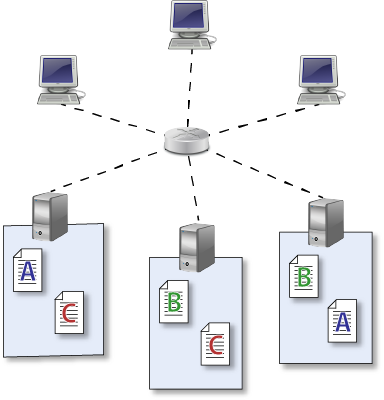
\includegraphics[width=\textwidth]{imagens/image1}
			\label{fig:exemplo}
		\end{figure}
		
		
		%\column{0.25\textwidth}
	\end{columns}
\end{frame}

\begin{frame}{}
	\begin{columns}
		\column{0.45\textwidth}
		
		\begin{figure}
			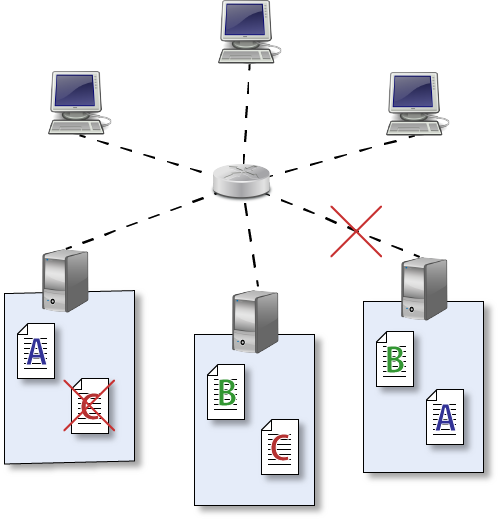
\includegraphics[width=\textwidth]{imagens/image2}
			\caption{Tolerância a falha}
			\label{fig:exemplo}
		\end{figure}
		
		\column{0.1\textwidth}
		
		\column{0.45\textwidth}
		
		\begin{figure}
			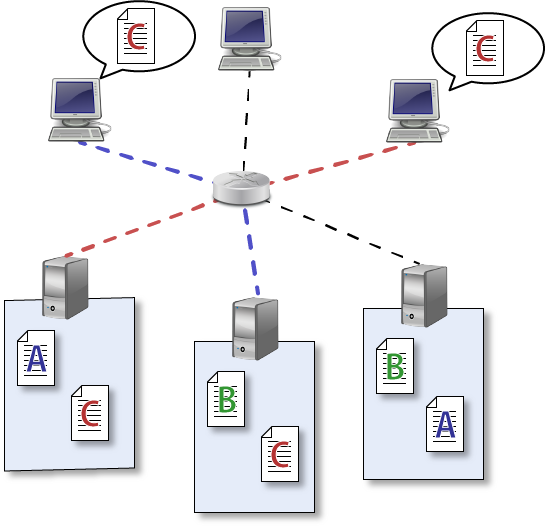
\includegraphics[width=\textwidth]{imagens/image3}
			\caption{Distribuição da carga}
			\label{fig:exemplo}
		\end{figure}
		
		
		%\column{0.25\textwidth}
	\end{columns}
\end{frame}

\begin{frame}{BFT-SMaRt}
	\begin{itemize}
		\item Biblioteca Java \textit{open-source}.
		\item Características:
		\begin{itemize}
			\item Replicação de máquina de estado (\textit{State Machine
				Replication - }SMR).
			\item Tolerante a falhas bizantinas (\textit{Byzantine Fault-Tolerant - BFT}).
			\item Simplicidade.
			\item Modularidade.
			\item API Simples e Extensível.
			\item Consciência de ambiente Multi-Core.	
			\item Reconfiguração.
		\end{itemize}
	\end{itemize}
\end{frame}

\begin{frame}{}		
	\begin{figure}
		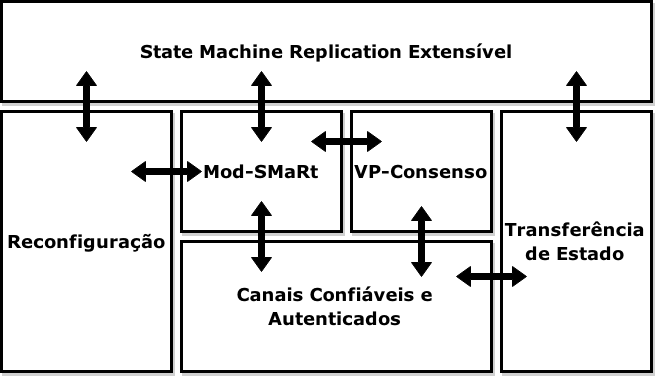
\includegraphics[width=\textwidth]{imagens/bftsmart1}
		\caption{Modularidade do BFT-SMaRt}
		\label{fig:bftsmart1}
	\end{figure}
\end{frame}

\begin{frame}{BFT-SMaRt}
	\begin{itemize}
		\item Para \textbf{n} réplicas e \textbf{f} falhas
		\begin{itemize}
			\item n $\geq$ 3f+1
			\begin{itemize}
				\item Falhas Bizantinas
			\end{itemize}
			\item n $\geq$ 2f+1
			\begin{itemize}
				\item Falhas de sistema
			\end{itemize}
		\end{itemize}
		\item Protocolos Centrais
		\begin{itemize}
			\item \textit{Total Order Multicast}	
			\item Transferência de Estados
		\end{itemize}
		
	\end{itemize}
\end{frame}

\begin{frame}{RAID}
	
	\begin{itemize}
		\item \textit{Redundant Array of Independent Disks}.
		\item Trata-se, basicamente, de uma solução computacional que combina vários discos rígidos (HDs) para formar uma única unidade lógica de armazenamento de dados.
	\end{itemize}
\end{frame}

\begin{frame}{RAID}
	
	\begin{itemize}
		\item Vantagens:
		\begin{itemize}
			\item Se um HD sofrer danos, os dados existentes nele não serão perdidos, pois podem ser replicados em outra unidade (redundância).
			\item É possível aumentar a capacidade de armazenamento a qualquer momento com a adição de mais HDs.
			\item O acesso à informação pode se tornar mais rápido, pois os dados são distribuídos a todos os discos.
			\item Dependendo do caso, há maior tolerância a falhas, pois o sistema não é paralisado se uma unidade parar de funcionar.
		\end{itemize}
	\end{itemize}
\end{frame}

\begin{frame}{RAID}
	\begin{itemize}
		\item Níveis de RAID
		\begin{itemize}
			\item RAID 0
			\item RAID 1
			\item RAID 5
		\end{itemize}
	\end{itemize}
\end{frame}

\begin{frame}{RAID 0}
	\begin{columns}
		\column{0.5\textwidth}
		\begin{itemize}
			\item Striping (fracionamento).
			\item Não oferece proteção contra falhas, pois não existe redundância.
			\item Focado no desempenho. Visto que quanto mais discos houver no sistema, maior é a sua taxa de transferência devido ao paralelismo nas operações de leitura e escrita.
		\end{itemize}
		
		\column{0.25\textwidth}
		\begin{figure}
			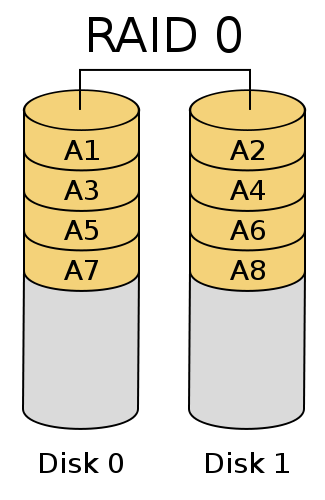
\includegraphics[width=\textwidth]{imagens/RAID_0}
			\label{fig:exemplo}
		\end{figure}
		
	\end{columns}
\end{frame}

\begin{frame}{RAID 1}
	\begin{columns}
		\column{0.5\textwidth}
		\begin{itemize}
			\item Mirror (Espelhamento).
			\item Necessita de uma quantidade par de discos.
			\item Vantagem
			\begin{itemize}
				\item Evita falhas físicas.
			\end{itemize}
			\item Desvantagens
			\begin{itemize}
				\item Perda de desempenho.
				\item Alto desperdício de espaço.
				\item  Não dispensa soluções de \textit{backup}.
			\end{itemize}
		\end{itemize}
		
		\column{0.25\textwidth}
		\begin{figure}
			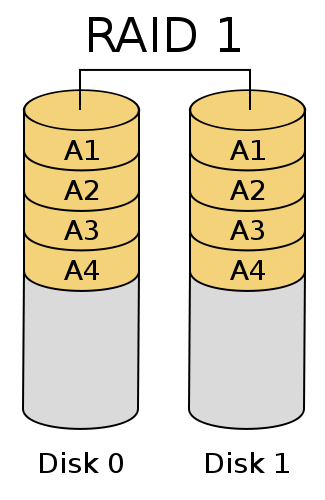
\includegraphics[width=\textwidth]{imagens/RAID_1}
			\label{fig:exemplo}
		\end{figure}
		
	\end{columns}
\end{frame}

\begin{frame}{RAID 5}
	\begin{columns}
		\column{0.5\textwidth}
		\begin{itemize}
			\item Esquema de paridade, pelo uso do bit de paridade.
			\item A informação sobre paridade é distribuída entre todos os discos.
			\item Vantagens
			\begin{itemize}
				\item Tolerância a falhas.
				\item Leitura rápida.
			\end{itemize}
			\item Desvantagens
			\begin{itemize}
				\item Sistema complexo de controle dos discos.
			\end{itemize}
		\end{itemize}
		
		\column{0.5\textwidth}
		\begin{figure}
			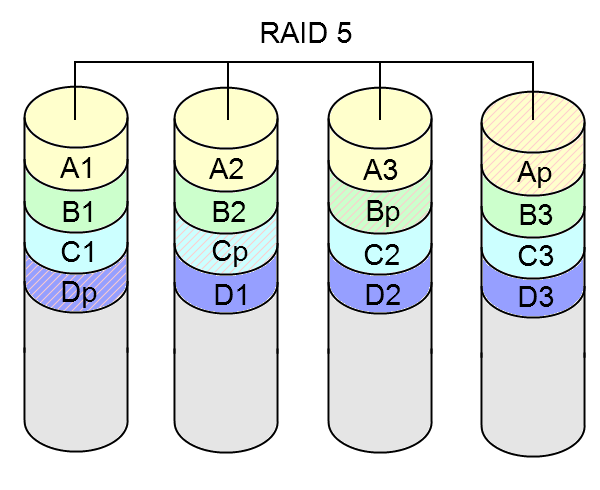
\includegraphics[width=\textwidth]{imagens/RAID_5}
			\label{fig:exemplo}
		\end{figure}
		
	\end{columns}
\end{frame}